\documentclass[tikz,border=10pt]{standalone}
\usepackage{tikz}
\usetikzlibrary{shapes,arrows,positioning}

\begin{document}
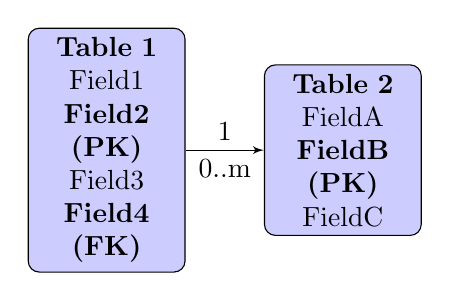
\begin{tikzpicture}[
    box/.style={rectangle, draw, fill=blue!20, text width=5em, text centered, rounded corners, minimum height=4em},
    node distance=3cm,
    arrow/.style={draw, -latex'}]

    % Node for the first table
    \node [box] (table1) {\textbf{Table 1}\\
                          Field1\\
                          \textbf{Field2 (PK)}\\
                          Field3\\
                          \textbf{Field4 (FK)}};

    % Node for the second table
    \node [box, right of=table1] (table2) {\textbf{Table 2}\\
                                           FieldA\\
                                           \textbf{FieldB (PK)}\\
                                           FieldC};

    % Draw the arrow with annotations
    \draw [arrow] (table1) -- node [midway, above] {1} node [midway, below] {0..m} (table2);
\end{tikzpicture}
\end{document}
